\documentclass{article}

% preambulo:
\usepackage[utf8]{inputenc}
% caracteres utf8 (tildes, enie) sin tener que usar comandos

\usepackage[spanish, es-tabla, es-nodecimaldot]{babel} 
% texto automatico en espaniol
% "tabla" en vez de "cuadro"
% no reemplaza puntos decimales por comas

%% NO AGREGAR PAQUETES ANTES DE ESTO, ES IMPORTANTE QUE BABEL ESTE PRIMERO

%%%%%%%%%%%%%%%%%%%%%%%%%%%%%%%%%
%% PAQUETES EXTRA %%%%%%%%%%%%%%%
%%%%%%%%%%%%%%%%%%%%%%%%%%%%%%%%%

\usepackage{subfiles}

\usepackage{amsmath} % PAQUETES DE MATEMATICA
\usepackage{amsfonts}
\usepackage{amssymb}

\usepackage{units} % permite usar nicefrac
\usepackage{graphicx} % importar imagenes
\usepackage{float} % posicion H para floats
\usepackage[colorinlistoftodos]{todonotes}


\usepackage[a4paper, total={6in, 8in}]{geometry}
\setlength{\parindent}{10pt}			%cuanta sangria al principio de un parrafo
\usepackage{indentfirst}				%pone sangria al primer parrafo de una seccion




%%%%%%%%%%%%%%%%%%%%%%%%%%%%%%%%%%%%%%%%%%%%%%%%%%%%%%%%%%%
%% NO AGREGAR PAQUETES DESPUES DE ESTO, ES IMPORTANTE QUE HYPERREF ESTE ULTIMO
\usepackage[hidelinks]{hyperref} % hipervinculos sin cajitas rojas




\begin{document}

\newgeometry{} % margenes default para la caratula
% caratula:
\begin{titlepage}
\newcommand{\HRule}{\rule{\linewidth}{0.5mm}}
\center
\mbox{\textsc{\LARGE \bfseries {Instituto Tecnol\'ogico de Buenos Aires}}}\\[1.5cm]
\textsc{\Large 22.12 Electr\'onica II}\\[0.5cm]


\HRule \\[0.6cm]
{ \Huge \bfseries Trabajo de laboratorio 1
\\ Fuente regulada de tensi\'on}\\[0.4cm] % Title of your document
\HRule \\[1.5cm]


{\large

\emph{Grupo 4}\\
\vspace{3px}

\begin{tabular}{lr} 	
\textsc{Bual\'o}, Santiago Andr\'es  & 57557 \\
\textsc{Laguinge}, Juan Mart\'in  & 57430 \\
\textsc{Martorell}, Ariel Antonio  & 56209 \\
\textsc{Parra}, Roc\'io  & 57669 \\
\end{tabular}

\vspace{20px}

\emph{Profesores}\\
\vspace{3px}
\textsc{Hirchoren}, Gustavo Abraham\\ 	
\textsc{Petrucci}, Javier David\\ 	

\vspace{100px}

\begin{tabular}{ll}

Presentado: & 23/04/2019\\

\end{tabular}

}

\vfill

\end{titlepage}

% indice:
\tableofcontents
\newpage


% cambio los margenes para el resto del documento
\newgeometry{total={6in, 8in}}
\subfile{e2_tp1_intro.tex}
\subfile{e2_tp1_protec.tex}

\begin{figure}[htp]
	\centering
	\fbox{
	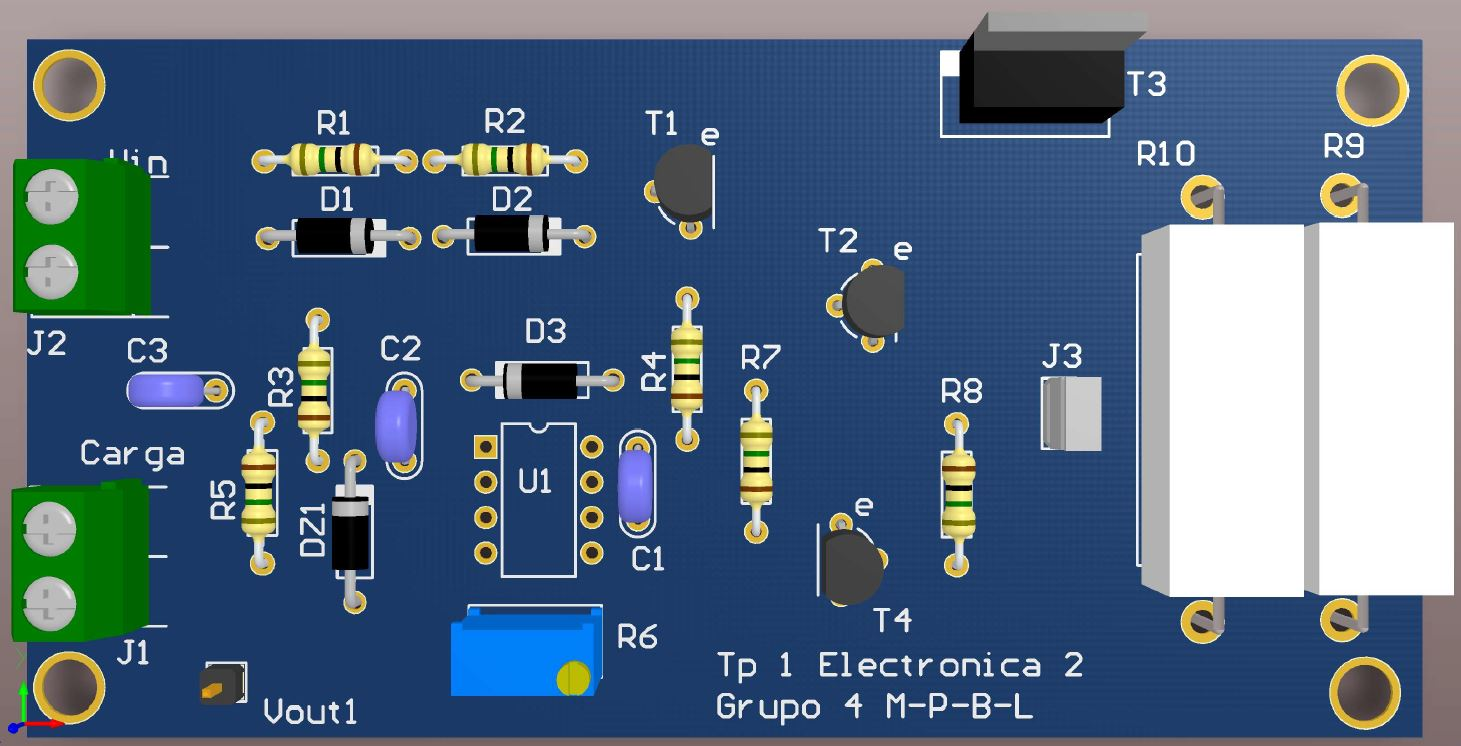
\includegraphics
	[width=\textwidth]
	{imagenes/pcb_3d_view.JPG}
	}
	\caption{3D del medelo del PCB dise\~nado}
	\label{fig:placa}
\end{figure}

\subfile{e2_tp1_barkhausen.tex}
\subfile{e2_tp1_disipador.tex}
\subfile{e2_tp1_carac_salida.tex}
\subfile{e2_tp1_ej1.tex}
\subfile{e2_tp1_ej2.tex}

\section{Conclusiones}

La fuente regulada de tensi\'on dise\~nada es capaz de regular correctamente entre 9V y 15V de salida, con hasta 1.5A de corriente.

La protecci\'on foldback del circuito logr\'o reducir a 1A la corriente con tensi\'on de salida 0. Siendo que incluso as\'i se podr\'ian disipar m\'as de 20W en el transistor de paso, y su temperatura aumentaba considerablemente incluso con un disipador de 3.5$\nicefrac{W}{^\circ C}$,  es razonable suponer que sin este tipo de protecci\'on no se habr\'ia podido evitar que se queme la placa en estas condiciones. Si bien eventualmente se llegar\'ia a un l\'imite por la m\'axima corriente que puede entregar la fuente de corriente al transistor de paso, como al dise\~nar se debe tener en cuenta los $\beta$ m\'inimos de los transistores, y estos tienen una gran dispersi\'on, tambi\'en es dif\'icil conseguir que la corriente m\'axima sea mayor que la que se desea como para garantizar que se pueda utilizar la carga m\'axima, pero no tanto mayor como para que se queme la placa. 
 




\clearpage

\end{document}
